\documentclass[12pt]{article}
\usepackage{setspace, indentfirst, hhline, graphicx, float, amssymb, amsmath, array, xcolor}
\usepackage[margin=1in]{geometry}

\newcolumntype{M}[1]{>{\centering\arraybackslash}m{#1}}

\newtheorem{thm}{Theorem}
\newtheorem{lem}[thm]{Lemma}

\begin{document}

\newcommand*{\titleGP}{\begingroup % Create the command for including the title page in the document
		\centering % Center all text
		\vspace*{\baselineskip} % White space at the top of the page

		\rule{\textwidth}{1.6pt}\vspace*{-\baselineskip}\vspace*{2pt} % Thick horizontal line
		\rule{\textwidth}{0.4pt}\\[\baselineskip] % Thin horizontal line

		{\LARGE AN EXPLORATION OF FAULHABER'S \\[0.2\baselineskip]}
		\vspace{0.7\baselineskip}
		{\LARGE FORMULA AND THE BERNOULLI NUMBERS}
		\\[0.2\baselineskip] % Title

\rule{\textwidth}{0.4pt}\vspace*{-\baselineskip}\vspace{3.2pt} % Thin horizontal line
\rule{\textwidth}{1.6pt}\\[1.5\baselineskip] % Thick horizontal line

\scshape % Small caps
MDM 4U7\\[0.7\baselineskip] 
\today \par % Location and year

\vspace*{2\baselineskip} % Whitespace between location/year and editors

By \\[0.7\baselineskip]
{\large ANDREW WANG\par} % Editor list

\vfill % Whitespace between editor names and publisher logo

\endgroup}

\titleGP
\newpage

\tableofcontents
\newpage

\setstretch{1.2}

\section{Introduction and Initial Exposure}
\subsection{Gauss}
\indent The story begins with a boy whose teacher was discontent with the class. As a result, the teacher punished his students by having them perform rote calculation and compelled them to calculate the sum of the first 100 positive integers. The activity was meant to take up the good part of an hour, but the boy only thought for a moment, after which he scribbled down his answer on the slate. He tossed the stone on his teacher's desk and rested as he waited for the others. The teacher said nothing, but was evidently skeptical, and so he decided that he would humiliate the boy later. Slowly, the students finished one by one, and after everyone had completed their work, the teacher turned the pile over. He was to look at the boy's first. Lo and behold, the boy's answer was 5050. The teacher's face flushed red in disbelief. Supposedly, that boy's name was Carl Friedrich Gauss. \\

The technique he used was relatively straight forward: he paired the first and last number, the second and second last, and so on, then summed the pairs. In fact, for a general arithmetic sequence with $n$ terms, starting term $a$, and common difference $d$, the technique still works. Namely, for
\begin{eqnarray*}
	S &=& a + (a + d) + (a + 2d) + \ldots + (a + (n - 2)d) + (a + (n - 1)d) \\
	&=& (a + (n - 1)d) + (a + (n - 2)d) + \ldots + (a + 2d) + (a + d) + a
\end{eqnarray*}
	
\noindent summing corresponding terms pairwise, vertically, yields $n$ terms, all equal to $2a + (n - 1)d$. Thus, after performing the addition this way, 

\begin{eqnarray*}
	2S &=& n(2a + (n - 1)d) \\
	\Rightarrow S &=& \frac{n}{2} (2a + (n - 1)d)
\end{eqnarray*}

for Gauss' instance of the problem, $a = 1$, $d = 1$, and 
\begin{eqnarray}
	S = \frac{n}{2}(2 + n - 1) = \frac{n}{2}(n + 1) = \frac{1}{2}n^2 + \frac{1}{2}n.
\end{eqnarray} Indeed, substituting $n = 100$ yields 5050. \\

My initial reaction to the story was one of awe. Gauss' clever exploitation of the commutative property of addition here was both ingenious and elegant, and this story is really what made me realize the importance of computational efficiency. As compared to the boy's classmates who had to sum the, say, $n$ terms, the simple formula would produce an answer in pretty well the same amount of time with $n = 100$ as $n = 10000$. 

But yet, I still was not satisfied. Why was the problem limited to the sum of the first $n$ numbers? What about their reciprocals? Their squares? Their cubes? Their $k^{th}$ powers? And so, I sought after a generalization.

\subsection{Sum of Squares}
At first, I looked into the sum of squares. I sought after a function $f(n)$, defined on the natural numbers, which would return the sum $1^2 + 2^2 + \ldots + n^2$ in some closed form. I took the most direct approach, which involved first constructing a table of values: 

\vspace{0.3\baselineskip}

\begin{center}
\begin{tabular}{|c|c|c|c|c|}
	\hline
	n & $\sum\limits_{i=1}^n i^2$ & $1^{st}$ difference & $2^{nd}$ difference & $3^{rd}$ difference \\ \hhline{|=|=|=|=|=|}
 	1 & 1 & & &\\ \hline
	2 & 5 & 4 & &\\ \hline
	3 & 14 & 9 & 5 &\\ \hline
	4 & 30 & 16 & 7 & 2\\ \hline
	5 & 55 & 25 & 9 & 2\\ \hline
	6 & 91 & 36 & 11 & 2\\ \hline
\end{tabular}
\end{center}

\begin{center}
\textbf{Table 1.} the first six sum of the squares of naturals and their differences.
\end{center}

\vspace{0.3\baselineskip}

The first observation I made was that it took three differences to reach a constant rate of change. A polynomial of degree three would also exhibit this property since differentiating three times would leave a constant. In fact, integrating three times the constant, 2, here yields $\frac{1}{3} x^3 + C$ where C is the constant of integration. The issue here is that all terms of degree less than 3 in the original polynomial would have contributed 0 to the third derivative of $f(n)$, and so those terms would be unknown when reversing the process. \\

At this point I did not see another way to approach the problem, so I took to Microsoft Excel's graphing software with the data in table 1. Sure enough, as can be seen in figure 1, after setting the equation to a polynomial of degree three, Excel produced the result $y = \frac{1}{3}x^3 + \frac{1}{2}x^2 + \frac{1}{6}x$. Of course, there was a constant here, but for the purpose of simplicity, I will say that the $3E-12$ term is negligible. 

\begin{center}
\begin{figure}[H]
	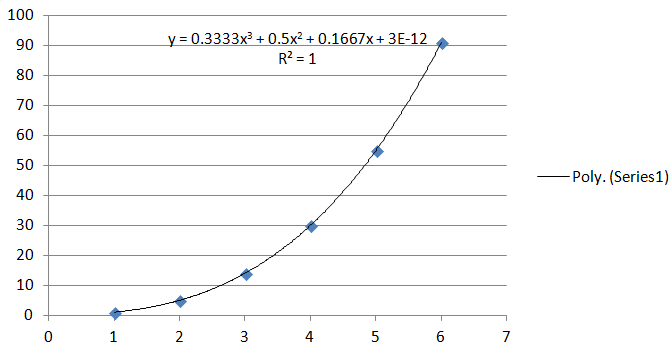
\includegraphics[scale=1.00]{squares.png}
\end{figure}
	\textbf{Figure 1.} $y = f(n)$.
\end{center}

But of course, this method feels like cheating. After looking through a bit of mathematical literature, sure enough, there was a proof of the above result. Notice its use of clever telescoping technique that reduces so that the desired sum is expressed in terms of other known sum(s) and, of course, $n$.

Since the desired sum is a cubic polynomial, start with the expansion, $$(n + 1)^3 = n^3 + 3n^2 + 3n + 1$$
\indent which, when rearranged to facilitate heavy cancellation, becomes, 
\begin{eqnarray}
	(n + 1)^3 - n^3 &=& 3n^2 + 3n + 1.
\end{eqnarray}
\indent Rewriting the above identity with $n - m,\  m \in \mathbb{N}$ in place of $n$ holds true as well. Namely, with $m \in \{1, 2, 3, \ldots , n - 2\}$,
\begin{eqnarray*}
	n^3 - (n-1)^3 &=& 3(n - 1)^2 + 3(n - 1) + 1 \\
	(n - 1)^3 - (n-2)^3 &=& 3(n - 2)^2 + 3(n - 2) + 1 \\
	&\vdots & \\
	3^3 - 2^3 &=& 3(2)^2 + 3(2) + 1 \\
	2^3 - 1^3 &=& 3(1)^2 + 3(1) + 1
\end{eqnarray*}

Adding all $n$ expressions on the left side and on the right, including $\left(2\right)$, yields
$$(n + 1)^3 - 1 = 3\displaystyle{\sum\limits_{i = 1}^n i^2} + 3\sum\limits_{i=1}^n i + \sum\limits_{i=1}^n 1$$.

Substituting (1), 
\begin{eqnarray*}
	3\sum\limits_{i=1}^n i^2 &=& n^3 + 3n^2 + 3n - 3\displaystyle{\left(\frac{(n)(n + 1)}{2}\right)} + n \\
	6\sum\limits_{i=1}^n i^2 &=& 2n^3 + 3n^2 + n \\
	&=& n(n + 1)(2n + 1)
\end{eqnarray*}
\begin{eqnarray}
	\therefore \sum\limits_{i=1}^n i^2 = \frac{n(n + 1)(2n + 1)}{6} = \frac{1}{3}n^3 + \frac{1}{2}n^2 + \frac{1}{6}n, \mathrm{\ as \ desired.}
\end{eqnarray}

\subsection{Sum of Cubes and then some}

I proceeded to work on the sum of cubes. This is one of the more interesting results. It turns out that 
\begin{eqnarray}
\sum\limits_{i=1}^n i^3 = \frac{1}{4}n^4 + \frac{1}{2}n^3 + \frac{1}{4}n^2 = \frac{n^2(n+1)^2}{4} = \left(\sum\limits_{i=1}^n i\right)^2.
\end{eqnarray}

\indent Incidentally, this result is often attributed to the Pythagorean, Nicomachus of Gerasa, who lived as early as c. 100 CE (Midonick, 1965, p. 15-6). \\

\indent After (4), it is possible to make two observations and possibly even a conjecture. The first is that for every sum of the $k^{th}$ powers of the natural numbers, the formula is a polynomial of degree $k + 1$. Next, the lack of a constant term in any of these formulae makes sense. When the upper bound, $n$, is 0, the sum of the $k^{th}$ powers of the first 0 numbers had better be 0. But here, in (4), there is not only no constant term but no linear term. Thus, it was proving to be difficult to spot an insightful pattern in the coefficient in these polynomials. \\

\indent Perhaps, with more cases, key insights might reveal themselves. From this point on, for the sake of convenience, define $S_k(n) = \sum\limits_{i=1}^n n^k$. Computing polynomials $S_k(n),\  k \in \{0, 1, 2, 3, 4, 5, 6 \}$ helps develop the following table of coefficients (Ezra, 2016):

\begin{table}[ht]
\centering
\begin{tabular}{| M{1cm} || M{1cm} | M{1cm} | M{1cm} | M{1cm} | M{1cm} | M{1cm} | M{1cm} | M{0.2cm}}
	\hline
	k & n & $n^2$ & $n^3$ & $n^4$ & $n^5$ & $n^6$ & $n^7$ \\[7pt] \hhline{|=|=|=|=|=|=|=|=|}
	0 & \textcolor{red}{$1$} & & & & & & \\[7pt] \hline
	1 & \textcolor{blue!70!cyan}{\large{$\frac{1}{2}$}} & \textcolor{red}{\large{$\frac{1}{2}$}} & & & & &\\[7pt] \hline
	2 & \large{$\frac{1}{6}$} & \textcolor{blue!70!cyan}{\large{$\frac{1}{2}$}} & \textcolor{red}{\large{$\frac{1}{3}$}} & & & & \\[7pt] \hline
	3 & \textcolor{orange!60!red}{0} & \large{$\frac{1}{4}$} & \textcolor{blue!70!cyan}{\large{$\frac{1}{2}$}} & \textcolor{red}{\large{$\frac{1}{4}$}} & & &\\[7pt] \hline
	4 & \textcolor{green!50!black}{\large{$-\frac{1}{30}$}} & \textcolor{orange!60!red}{0} & \large{$\frac{1}{3}$} & \textcolor{blue!70!cyan}{\large{$\frac{1}{2}$}} & \textcolor{red}{\large{$\frac{1}{5}$}} & &\\[7pt] \hline
	5 & \textcolor{orange!60!red}{0} & \textcolor{green!50!black}{\large{$-\frac{1}{12}$}} & \textcolor{orange!60!red}{0} & \large{$\frac{5}{12}$} & \textcolor{blue!70!cyan}{\large{$\frac{1}{2}$}} & \textcolor{red}{\large{$\frac{1}{6}$}} & \\[7pt] \hline
	6 & \large{$\frac{1}{42}$} & \textcolor{orange!60!red}{0} & \textcolor{green!50!black}{\large{-$\frac{1}{6}$}} & \textcolor{orange!60!red}{0} & \large{$\frac{1}{2}$} & \textcolor{blue!70!cyan}{\large{$\frac{1}{2}$}} & \textcolor{red}{\large{$\frac{1}{7}$}} \\[7pt] \hline
\end{tabular}
\end{table}
\begin{center}
	\textbf{Table 2.} Coefficients of $S_k(n),\  k \in \{0, 1, 2, 3, 4, 5, 6 \}$.
\end{center}

\indent Now, there are four observations that can be made. First, the leading coefficient (in red) in each instance of $S_k$ is simply the reciprocal of $k + 1$. Second, for $k \geq 1$, the coefficient of the second highest degree term (in blue) is consistently $\frac{1}{2}$. Third, It appears that for odd $k \geq 3$, there is no linear term. All the orange 0's form a diagonal, too. Finally, the coefficients in the green diagonal are all negative. \\

\indent At this point in my exploration, I am finding it increasingly tedious to compute the polynomials with the method from before. Furthermore, the method requires that all sum formulas below the desired power be known. Thus, the previous issue of computational inefficiency Gauss so cleverly avoided has once again presented itself in this extension of the problem. Finally, then, we inquire whether there is a closed form of $S_m(n) \ , m \in \mathbb{N}$.  \\

But first, we observe the telescoping method's generalization, so to speak, for $S_m(n)$: \\

\indent Begin with the expansion of $(n + 1)^{m + 1}$, 
\begin{eqnarray*}
	(n + 1)^{m + 1} &=& n^{m + 1} + (m + 1)n^m + \binom{m + 1}{2}n^{m - 1} + \binom{m + 1}{3}n^{m - 2} + \ldots + 1 \\
	(n + 1)^{m + 1} - n^{m + 1} &=& (m + 1)n^m + \binom{m + 1}{2}n^{m - 1} + \binom{m + 1}{3}n^{m - 2} + \ldots + 1 \\	
\end{eqnarray*} 

\indent replacing $n$ with $n - 1$, $n - 2$, \ldots, $2$, $1$ will also satisfy the identity:

\begin{eqnarray*}
n^{m + 1} - (n-1)^{m + 1} &=& (m + 1)(n - 1)^m + \binom{m + 1}{2}(n-1)^{m - 1} + \\ 
&\ &\binom{m + 1}{3}(n-1)^{m - 2} + \ldots + 1 \\	
(n - 1)^{m + 1} - (n-2)^{m + 1} &=& (m + 1)(n -2)^m + \binom{m + 1}{2}(n-2)^{m - 1} + \\
&\ &\binom{m + 1}{3}(n-2)^{m - 2} + \ldots + 1 \\
&\vdots & \\
3^{m + 1} - 2^{m + 1} &=& 2^m(m + 1) + \binom{m + 1}{2}2^{m - 1} + \binom{m + 1}{3}2^{m - 2} + \ldots + 1 \\
2^{m + 1} - 1^{m + 1} &=& (m + 1)1^m + \binom{m + 1}{2}1^{m - 1} + \binom{m + 1}{3}1^{m - 2} + \ldots + 1 \\
\end{eqnarray*}

\indent Again, adding all $n$ expressions on the left sides and those on the right sides causes heavy cancellation:

\begin{eqnarray*}
(n + 1)^{m + 1} - 1 &=& (m + 1)S_m(n) + \binom{m + 1}{2}S_{m - 1}(n) + \binom{m + 1}{3}S_{m - 2}(n) \ldots + S_0(n) \\ 
&=& (m + 1)S_m(n) + \sum\limits_{i = 1}^m \binom{m + 1}{i + 1} S_{m - i} (n) \\
&=& \sum\limits_{j = 1}^{m + 1} \binom{m + 1}{j} n^{m + 1 - j} - 1\\
\end{eqnarray*}
\begin{equation}
	S_m(n) = \left(\frac{1}{m + 1}\right)\left(\sum\limits_{j = 1}^{m + 1} \binom{m + 1}{j} n^{m + 1 - j} - \sum\limits_{i = 1}^m \binom{m + 1}{i + 1} S_{m - i} (n) - 1\right).
\end{equation}

\vspace{0.6\baselineskip}

A rather monstrous result, really. 

\section{Generalizations}

\indent Johann Faulhaber of Ulm (1580-1635) devoted a substantial part of his life to this very problem|he notably calculated the sum formulas of odd powers up to 17 (Knuth, 1993, p.277-8). In particular, he defined $N = \frac{n^2 + n}{2}$ and expressed all the sum formulas as polynomials in $N$. \\

It was after Johann Faulhaber that the Faulhaber formula was named, though the result is more accurately ascribed to Jacob Bernoulli and, simultaneously, Takakazu Seki (Beery, 2010). Indeed, the closed form expression given by Bernoulli features the Bernoulli numbers: a sequence of which Faulhaber likely had no knowledge seeing as Bernoulli discovered it after Faulhaber had past away. \\

Therefore, since the closed form formula involves the Bernoulli numbers, there ought to be a brief discussion on the sequence.

\subsection{The Bernoulli Numbers}

The Bernoulli numbers, $B_n$ are a sequence of rational numbers whose appearances in the world of number theory are plentiful, for instance, the Basel problem (Sullivan, 2013). \\

By definition, 
$$\sum\limits_{i = 0}^m \binom{m + 1}{i} B_i = 0$$
\indent and  $B_0$ = 1. $m$ is chosen as needed. Indeed,  $B_1$ can be computed by letting $m = 1$:

$$\binom{2}{0}B_0 + \binom{2}{1}B_1 = 0 = 1 + 2B_1 \Rightarrow B_1 = -\frac{1}{2}.$$

By repeating this process, we can produce the first 7 Bernoulli numbers: 

\begin{table}[ht]
\centering
\begin{tabular}{|M{1cm}|M{1cm}|}
	\hline
	n & $B_n$ \\ \hhline{|=|=|}
	0 & 1 \\ \hline
	1 & \large{$-\frac{1}{2}$} \\ \hline
	2 & \large{$\frac{1}{6}$} \\ \hline
	3 & 0 \\ \hline
	4 & \large{$-\frac{1}{30}$} \\ \hline
	5 & 0 \\ \hline
	6 & \large{$\frac{1}{42}$} \\ \hline
\end{tabular}
\end{table}
\begin{center}
	\textbf{Table 3.} the first 7 Bernoulli numbers.
\end{center}

These numbers look familiar. In fact, they are the coefficients of the linear terms in table 2! The one difference is that $B_1$ is negative. This is a discrepancy that is addressed by the "first" and "second" Bernoulli numbers. The difference between the two is only $B_n$, where the first Bernoulli numbers, $B^-_n$, are such that $B_1 = -\frac{1}{2}$. The second Bernoulli numbers have $B_1 = +\frac{1}{2}.$ Both work, but by convention the first Bernoulli numbers are used. The difference in the end is simply that the formula would contain $(-1)^{j}$ so that all odd Bernoulli numbers have their signs switched. However, the odd Bernoulli numbers, $B_k \ k\geq 3$, are all zero, and so that the $-1$ effectively only changes $B_1$. I will examine the version with the second Bernoulli numbers.

\subsection{Faulhaber's Formula}

Faulhaber's formula states that: 
$$S_m(n) = \frac{1}{m + 1} \sum\limits_{i = 1}^m \binom{m + 1}{k} B_k n^{m + 1 - k}$$.

The derivation I considered is from Aigner's "A Course in Enumeration" (Springer, 2007). It is very involved, and so only the overview will be provided. \\

\textbf{Lemma 1} Let $a_n$ and $b_n$ be two sequences not necessarily unique. Define $\hat{A}(z) = \sum\limits_{n \geq 0} a_n \frac{z^n}{n!}$ and $\hat{B}(z) = \sum\limits_{n \geq 0} b_n \frac{z^n}{n!}$. $\exists \hat{D}(z) = \sum\limits_{n \geq 0} d_n \frac{z^n}{n!} = (\hat{A}(z))(\hat{B}(z))$, where $d_n = \sum\limits_{i = 0}^n \binom{n}{i} a_i b_{n - i}$. \\

This result makes more sense when the sums are written out in full: 
$$(\frac{a_0}{0!}z^0 + \frac{a_1}{1!}z^1 + \frac{a_2}{2!}z^2 + \ldots)(\frac{b_0}{0!}z^0 + \frac{b_1}{1!}z^1 + \frac{b_2}{2!}z^2 + \ldots) = \frac{a_0b_0}{0!0!} z^0 + \left(\frac{a_0 b_1}{0!1!} + \frac{a_1b_0}{1!0!}\right)z^1 + \left(\frac{a_0b_2}{0!2!} + \ldots + \frac{a_2b_0}{2!0!}\right)$$

By matching each coefficient, $c_i$, by powers of $z$, we see that $$c_i = \sum\limits_{i = 0}^k \frac{a_ib_{k-i}}{i!(k - i!)}$$. 

After defining $d_i = (k!)c_i$ and simplifying, lemma 1 is proved.

The derivation then looks at $S_m(n)$, though it is defined slightly differently from what I had, previously. Here, we redefine $S_m(n)$ with upper bound $n - 1$ instead of $n$.

After defining $\hat{S}(z) = \sum\limits_{m \geq 0} S_m(n) \frac{z^m}{m!}$ and manipulating this generating function by observing the presence of the Maclaurin series of $e^x$ (Weisstein, result 14), we arrive at: 

\begin{equation*}
	\hat{S}(z) = \frac{e^{nz} - 1}{e^z - 1}.
\end{equation*}

Next, we observe that the numerator is very close to the exponential generating function for the $nz^{th}$ powers of $e$, differing only by the $-1$. Thus, we define

\begin{eqnarray*}
	\hat{P}_n(z) &=& \sum\limits_{m \geq 0} n^m \frac{z^m}{m!} \\
	&=& e^{nz}.
\end{eqnarray*}

A part of the proof that is omitted for now is the result: that the generating function of the Bernoulli numbers is

$$\hat{B}(z) = \sum\limits_{n \geq 0}B_n \frac{z^n}{n!} = \frac{z}{e^z - 1}.$$

This result is shown with lemma 1 and a manipulation of the definition of the Bernoulli numbers provided in \textbf{2.1}. \\

Nonetheless, we arrive at $$(\hat{P}_n(z) - 1)(\hat{B}(z)) = z\hat{S}(z).$$

Now that there are two unique expressions of the same entity, we may compare them. Namely, by matching the coefficients of the $z^{m + 1}$ terms and isolating $S_m$, the formula is proven. 

\newpage
\begin{thebibliography}{3}
\bibitem[1]{Beery}
	
	Beery, Janet. (University of Redlands), "Sums of Powers of Positive Integers," Convergence (July 2010), DOI:10.4169/loci003284
	
\bibitem[2]{Getzler}
	Getzler, Ezra. (2016). The Bernoulli Numbers [PowerPoint slides]. Retrived from https://www.youtube.com/watch?v=UALayaK5mMU

\bibitem[3]{Knuth}
	Knuth, D. (1993). Johann Faulhaber and Sums of Powers. Mathematics of Computation, 61(203), 277-294. doi:10.2307/2152953
	
\bibitem[4]{Midonick}
Midonick, Henrietta (1965), The Treasury of Mathematics, Volume 2, pages 15-16. Penguin Books.
\bibitem[5]{Kolbert}
	Kolbert, E. 
	(2011, August 15). 
	Sleeping with the Enemy.
	Retrieved May 03, 2016, 
	from http://www.newyorker.com/magazine/2011/08/15/sleeping-with-the-enemy

\bibitem[6]{Wolfram}
	Weisstein, Eric W. "Maclaurin Series." From MathWorld--A Wolfram Web Resource. http://mathworld.wolfram.com/MaclaurinSeries.html

\end{thebibliography}


\end{document}